\documentclass[conference]{IEEEtran}
\IEEEoverridecommandlockouts
% The preceding line is only needed to identify funding in the first footnote. If that is unneeded, please comment it out.
\usepackage{cite}
\usepackage{amsmath,amssymb,amsfonts}
\usepackage{algorithmic}
\usepackage{graphicx}
\usepackage{textcomp}
\usepackage{xcolor}
\usepackage{hyperref}
\usepackage{amsmath}
\usepackage{amssymb}

\newcommand{\rom}[1]{\uppercase\expandafter{\romannumeral #1\relax}}

\DeclareMathOperator*{\argmin}{arg\,min}

\def\BibTeX{{\rm B\kern-.05em{\sc i\kern-.025em b}\kern-.08em
    T\kern-.1667em\lower.7ex\hbox{E}\kern-.125emX}}
\begin{document}

\title{Assignment 4: a mathematical essay on decision tree\\}


\author{\IEEEauthorblockN{Gautham Govind A}
\IEEEauthorblockA{\textit{Dept. of Electrical Engineering}\\
\textit{Indian Institute of Technology Madras} \\}
\textit{ee19b022@smail.iitm.ac.in}

}

\maketitle

\begin{abstract}
The objective of this assignment is to explore the mathematical formalism behind decision tree classifier and then to use it in a real-life application. In this assignment, as a real-life application, decision tree classifier is used to formally identify the factors which could have been used to predict how acceptable a car is from the popular car evaluation dataset. Data visualization, cleaning and modelling is done using Python. The analysis enables us to arrive at the conclusion that it is possible to make reasonable predictions regarding the acceptability of a car using factors including but not limited to safety rating, price and luggage boot space. 
\end{abstract}

\begin{IEEEkeywords}
decision tree, python, visualization, predictive modelling, multinomial classification
\end{IEEEkeywords}

\section{Introduction}

Given a set of features and a target variable, predictive modelling is typically used for generating a model which can make predictions for cases where we do not know the value of the target variable, i.e., only the features are available. Apart from this use, a model can also be used for developing an intuition of how various factors influence the target variable. In this assignment, we try to make use of a model for the purpose of identifying the key factors which influence the decision in a classification problem.

In particular, we make use of decision tree classifier for the purpose of identifying relationships in a classification problem. Decision trees are among the most popular machine learning algorithms given their intelligibility and simplicity.. Though they are by nature very simple, they can give good, and more importantly, interpretable results in many problem settings. Decision tree is a very flexible classifier in the sense that it can accommodate both continuous and categorical variables. In our particular problem, we will restrict ourselves to a classification problem using categorical variables.


In our problem setting, the goal is to use decision tree classifier to predict the acceptability level of a car given a variety of factors like price, number of doors, passenger capacity, luggage boot space and safety rating. We make use of the publicly available car evaluation dataset for building the model. After building the model, we evaluate the model using a variety of evaluation metrics. By examining how well the model performs, we can identify how good the identified relationships are. Also, we check how critical each feature is to the prediction and create a ranking based on the importance of features.


Section \rom{2} gives an overview of the various techniques used for data cleaning, data visualization and an initial exploratory analysis. A lot of insights can be gained just by making qualitative observations from the given data. Section \rom{3} gives a short description of the mathematical formalism behind decision tree. Section \rom{4} describes the various models that were tried and the results that were obtained by applying decision tree in this particular case. Section \rom{5} gives a summary of the major conclusions drawn from the analysis.


\section{Exploratory Data Analysis}

In this section, we describe the process of data cleaning and data visualization. We also make some qualitative observations.

\subsection{Preliminary analysis}

The given dataset has 1728 rows and 7 columns. It must be noted that the dataset itself lacked any column headings: they had to be added in manually. A brief overview of the dataset is presented in Figure \ref{df_info}. We observe that we have \textbf{only categorical variables.} It also seems that there are no null values. 

We also look at the distribution for our target class, which is the acceptability rating termed 'target'. On plotting, we obtain Figure \ref{target_dist}. We have four categories: unacc (Unacceptable), acc (Acceptable), good (Good) and vgood (Very good). The count of cars in the unacceptable category is disproportionately high compared to other categories. We will have to account for this during model building.

\begin{figure}[tbh]
\centering
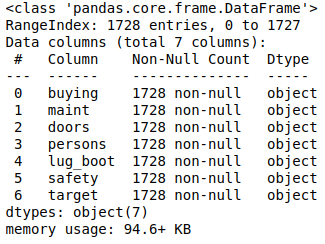
\includegraphics[scale = 0.50]{df_info.png}
\caption{Summary of the dataset}
\label{df_info}
\end{figure}

\begin{figure}[tbh]
\centering
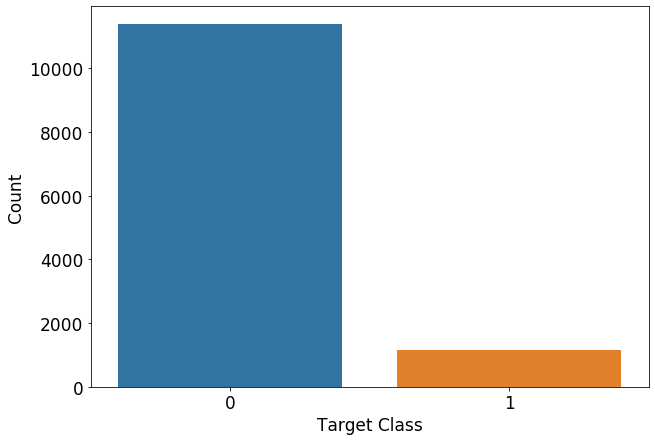
\includegraphics[scale = 0.39]{target_dist.png}
\caption{Target class imbalance}
\label{target_dist}
\end{figure}

\subsection{Feature by feature analysis}

Since all 6 features are categorical, for each feature we create a count plot, separating out the target classes. This can give qualitative insights regarding how a feature may affect the target variable. 

\subsection*{Buying price}

We obtain the count plot as shown in Figure \ref{bp}. We make the following observations:

\begin{itemize}
    \item Cars with high and very high buying price have a large proportion of unacceptable vehicles. Furthermore, there are no good or very good vehicles at this price range.
    \item Medium and low priced cars have representation from all four target categories.
\end{itemize}

Intuitively, this makes sense since people generally tend to find high prices unacceptable. For a deal to be considered good/ very good, it is almost always the case that the price should be on the lower end.

\begin{figure}[tbh]
\centering
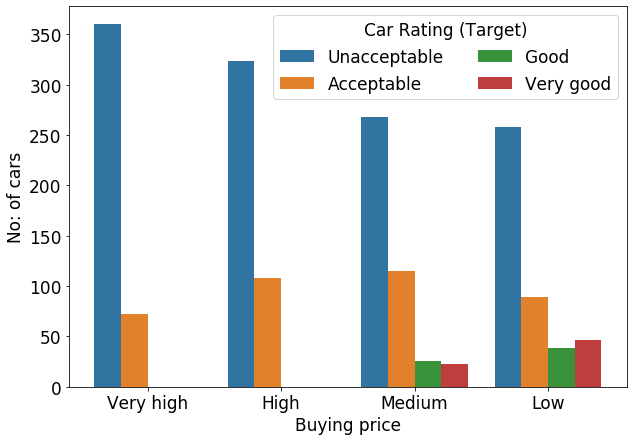
\includegraphics[scale = 0.39]{bp.png}
\caption{Distribution of buying price}
\label{bp}
\end{figure}

\subsection*{Maintenance price}

We obtain the count plot as shown in Figure \ref{mp}. We observe that the distribution is largely identical to the distribution for buying price. Again, we expect people to find high maintenance cost to be generally unacceptable.  

\begin{figure}[tbh]
\centering
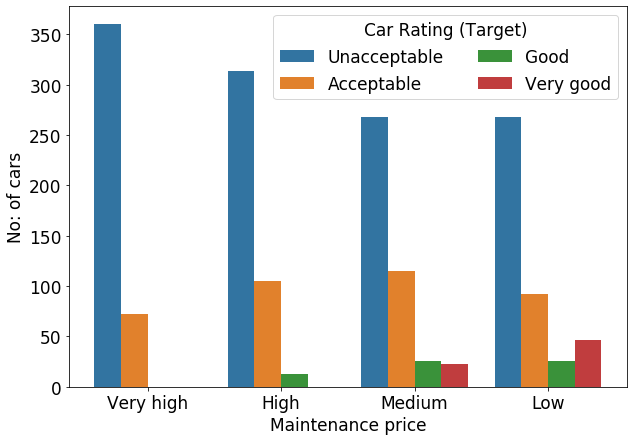
\includegraphics[scale = 0.39]{mp.png}
\caption{Distribution of maintenance price}
\label{mp}
\end{figure}

\subsection*{Number of doors}

We obtain the count plot as shown in Figure \ref{nd}. We observe that the distribution is largely identical for each category, i.e., irrespective of what the number of doors is, the distribution is same. In other words, the number of doors doesn't really provide any information regarding what would be the acceptability rating of a car. This implies that number of doors is not really a deciding factor as far as acceptance rating is concerned.

\begin{figure*}[tbh]
\centering
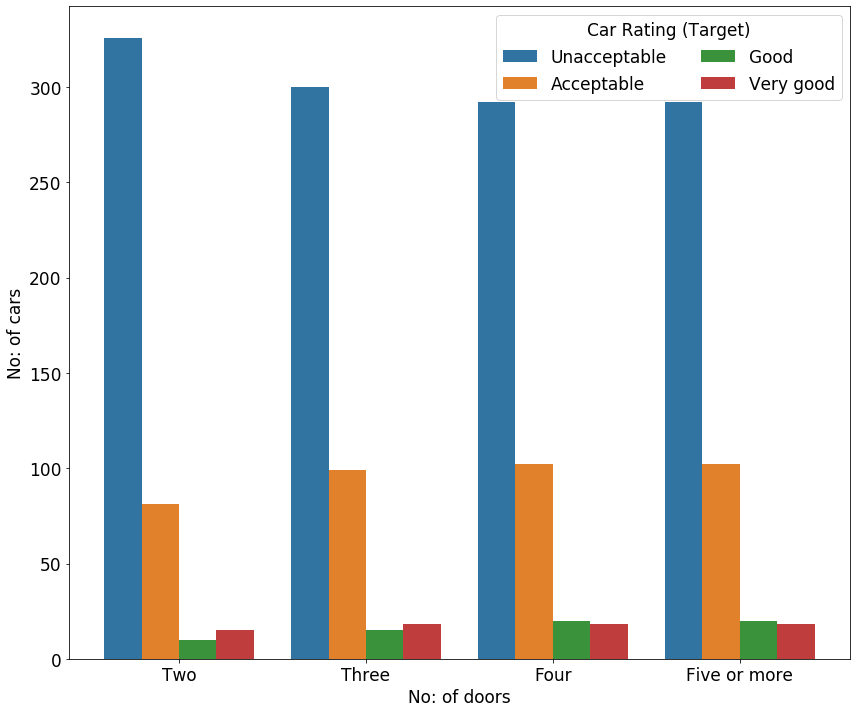
\includegraphics[scale = 0.4]{nd.png}
\caption{Distribution of number of doors}
\label{nd}
\end{figure*}

\subsection*{Passenger capacity}

We obtain the count plot as shown in Figure \ref{cp}. We make the following observations:

\begin{itemize}
    \item Cars that can accommodate only two people are all unacceptable.
    \item Cars which can accommodate four and more than four have similar distributions.
\end{itemize}

This seems to suggest that while having at least 4 seats is essential, beyond that the number of seats doesn't really have an impact on the acceptability rating.

\begin{figure}[tbh]
\centering
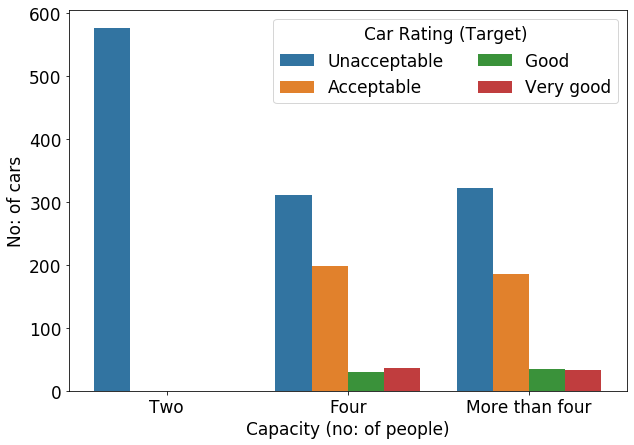
\includegraphics[scale = 0.39]{cp.png}
\caption{Distribution of passenger capacity}
\label{cp}
\end{figure}

\subsection*{Size of luggage boot}

We obtain the count plot as shown in Figure \ref{lgp}. We observe that though all categories have representation from all target categories, in general, the rating increases as the luggage boot size increases, which is what we would expect intuitively anyway.

\begin{figure}[tbh]
\centering
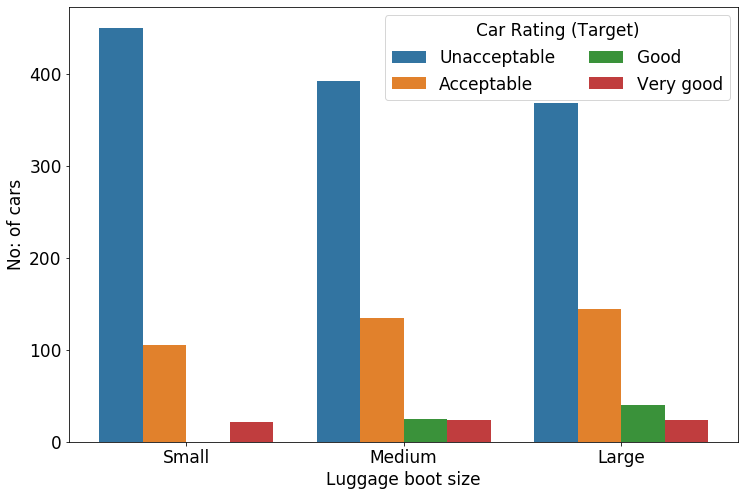
\includegraphics[scale = 0.33]{lgp.png}
\caption{Distribution of luggage boot size}
\label{lgp}
\end{figure}

\subsection*{Safety rating}

We obtain the count plot as shown in Figure \ref{sfp}. We make the following observations:

\begin{itemize}
    \item All low safety rated cars are unacceptable, which is what we would expect.
    \item As safety level increases, proportion of unacceptable cars decreases.
\end{itemize}

This seems to suggest that safety is a strong factor in predicting the acceptability of a car.

\begin{figure}[tbh]
\centering
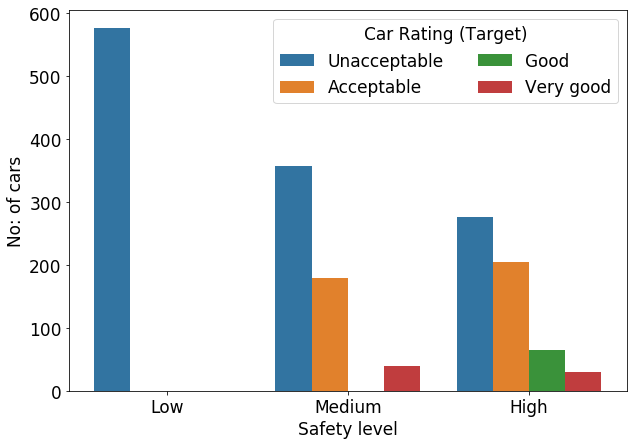
\includegraphics[scale = 0.39]{sfp.png}
\caption{Distribution of safety levels}
\label{sfp}
\end{figure}



\section{Model: Naive Bayes Classifier}

In this section, we will give a brief overview of the mathematical formalism behind the decision tree classifier. 

In general, decision trees come under the broad umbrella of algorithms called CART algorithms: Classification and Regression Tree algorithms. Decision tree is a specific algorithm within this broad class. Decision trees themselves are of two kinds:
\begin{enumerate}
    \item Classification trees: When the predicted outcome is the class (discrete) to which the data belongs.
    \item Regression trees:  When the predicted outcome can be considered a real number.
\end{enumerate}
In this assignment, we will be making use of classification trees since the problem is a multi-label classification problem.

\subsection{Algorithm Overview}

Before describing the algorithm used by a decision tree classifier, it is necessary to make oneself familiar with the terminology and structure of a decision tree. A prototypical decision tree is shown in Figure \ref{decision_tree}. A brief overview of the terminology:
\begin{itemize}
    \item Root node: Root node is from where the decision tree starts. It represents the entire dataset.
    \item Decision node: Decision node represents a node where a decision has to be made regarding a split to the dataset under current consideration.
    \item Leaf node: Leaf node represents the final output node. The tree cannot be segregated further after reaching a leaf node.
\end{itemize}

\begin{figure}[tbh]
\centering
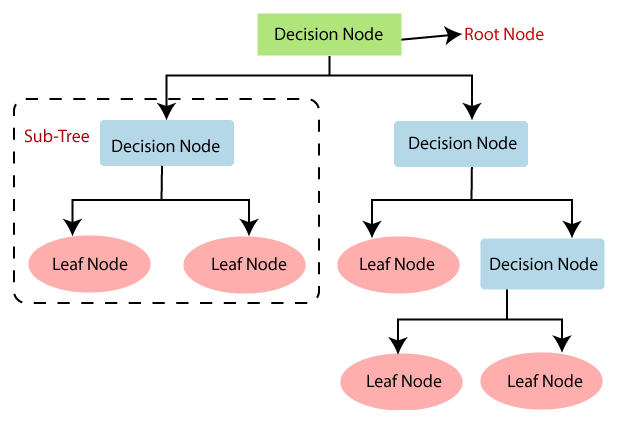
\includegraphics[scale = 0.39]{decision_tree.png}
\caption{Structure of a decision tree}
\label{decision_tree}
\end{figure}

A decision tree classifier makes used of a \textbf{rule-based classification algorithm} as opposed to a probabilistic model, which is adopted by algorithms like naive bayes. This means that rather than learning a number of parameters and then using this for predicting the probability of a sample belonging to a particular class, a set of learnt rules are used for directly predicting the class of a sample. In a sense, this rule-based approach mimics human decision making process.

The general structure of the algorithm used by a decision tree classifier is outlined below:

\begin{enumerate}
    \item Begin the tree with the root node which contains the complete dataset. 
    \item Find the best attribute in the dataset using Attribute Selection Measure (ASM). More details regrading ASM will be discussed in the following section.
    \item Split the dataset my making a decision rule based on an optimal value of the best attribute.
    \item Recursively make new decision trees using the subsets of the dataset created in step 3. Continue this process until you reach a leaf node. 
\end{enumerate}

Once the tree has been built, classifying a new sample is as simple as traversing the tree till you reach a leaf node, which will provide the predicted class. 

The major benefits offered by a decision tree classifier are:
\begin{itemize}
    \item \textbf{Uses a white box/open-box model:} If a given situation is observable in a model the explanation for the condition is easily explained by boolean logic. By contrast, in a black box model, the explanation for the results is typically difficult to understand, for example with an artificial neural network.
    \item \textbf{Non-parametric approach}: Makes no assumptions of the training data or prediction residuals; e.g., no distributional, independence, or constant variance assumptions.
    \item \textbf{Requires little data preparation}: Other techniques often require data normalization. Since trees can handle qualitative predictors, there is no need to create dummy variables
\end{itemize}

Some limitations of this approach:
\begin{itemize}
    \item \textbf{Trees are unstable:} A small change in the training data can result in a large change in the tree and consequently the final predictions.
    \item \textbf{Non-optimality}: Practical decision-tree learning algorithms are based on heuristics such as the greedy algorithm where locally optimal decisions are made at each node. Such algorithms cannot guarantee to return the globally optimal decision tree.
\end{itemize}

\subsection{Mathematical formalism}

What a decision tree essentially learns is a decision for each decision node. In particular, suppose a decision tree makes use of an impurity measure S (various measures for quality will be discussed). Suppose a node splits the dataset into two subsets left and right. Then the node computes the quantity:
$$ J(k, t_k) = \frac{m_\textrm{left}}{m}G_\textrm{left} + \frac{m_\textrm{right}}{m}G_\textrm{right} $$ where $m_\textrm{left}$ is the number of samples in the left subset, $m_\textrm{right}$ is the number of samples in the right subset, $S_\textrm{left}$ is the impurity measure for the left subset and $S_\textrm{right}$ is the impurity measure for the right subset. The attempt is to find the split which minimizes $J(k, t_k)$.

We can regard $J(k, t_k)$ as the cost function. The algorithm first splits the training set into 2 subsets using a single feature $k$ and a threshold $t_k$ . A pair $(t_k , k)$ is searched that minimizes the cost function the best. This procedure is repeated, looking for the best predictor and the best cut-point in order to split the data further so as to minimise the cost function. This process
continues till the set stopping criterion is reached or when every training sample is perfectly classified.

It is to be noted that without the intervention of appropriate stopping criterion or other means, the tree could grow very deep, leading to over-fitting. Decision Trees are also unstable, meaning trees learnt from different samples of a dataset are likely to differ in their structure compared to approaches such as logistic regression or naive bayes.

An overview of two common attribute selection measures/ impurity measures is given below:

\begin{enumerate}

    \item Gini Index/Impurity: This is essentially a measure of total variance across the K classes.
    $$ G = \sum_{k=1}^{K}\hat{p_{i, k}}(1 - \hat{p_{i, k}}) $$ where $p_{i,k}$ is the ratio of class k instances among the training instances in the ${i^\textrm{th}}$ node. The Gini index takes on a small value if all of the $\hat{p}_{i,k}$ ’s are close to zero or one. So, small value implies that a node predominantly contains one class. And a zero value implies that the node is pure. Thus Gini index could also be viewed as a measure of impurity. The equation for Gini index can also be rewritten as:
    $$ G = 1 - \sum_{k=1}^{K}\hat{p_{i, k}^2} $$
    
    \item Entropy: The formulation has a close resemblance with the entropy formulation in thermodynamics. 
    $$ D = -\sum_{k = 1}^{K}\hat{p_{i, k}}\log{\hat{p_{i, k}}} $$ where again K is the total number of classes and $p_{i,k}$ is the ratio of class k instances among the training instances in the ${i^\textrm{th}}$ node. As was the case with Gini index, a smaller value of entropy signifies higher purity and a larger value of entropy signifies impurity.
\end{enumerate}



\subsection{Regularization techniques}

As discussed above, allowing a tree to grow without stopping condition will inevitable lead to over-fitting. To mitigate this, we generally apply regularization techniques so as to increase the ability of the mode to generalize. We effectively tune the low bias - high variance model such that we decrease the variance at the cost of slightly increasing the bias. Two common regularization techniques are discussed below:

\begin{enumerate}
    \item \textbf{Cost-complexity pruning:} Rather than considering every possible sub-tree, we consider a sequence of trees indexed by non-negative tuning parameter $\alpha$. For each $\alpha$, these correspond to a sub-tree $T \in T_0$ such that $$ J(k, t_k) + {\alpha}|T| $$ is as small as possible. Here $|T|$ indicates the number of terminal nodes of a tree. Notice that if $\alpha = 0$, the sub-tree $T$ is the original tree $T_0$ . We can select a value for $\alpha$ using a validation set or cross-validation.
    \item \textbf{Bagging:} In bagging, we construct B trees using B bootstrapped training sets and average the resulting predictions. Bootstrapping is a technique to obtain datapoints using random sampling with replacement. Although the constructed trees may be deep and hence suffer from high variance individually, averaging reduces variance and results in a better model. This, in fact, is a precursor to Random forests which in addition to this, deploys random features during splitting . Bagging improves prediction by lowering the variance, but at the expense of loss of interpretability.
\end{enumerate}



\section{Modelling }

In this section, we discuss the application of the decision tree classifier to our problem. 

We create and evaluate three models:

\begin{enumerate}
    \item In Model 1, we let the decision tree grow without any constraints.
    \item In Model 2, we perform pruning on the tree to avoid overfitting.
    \item In Model 3, we perform bagging to avoid overfitting.
\end{enumerate}

For each model, we take care to account for the inherent imbalance in the training dataset with respect to the target class. This is done by making use of appropriate wweights during the training of the decision tree.

We evaluate the models based on multiple metrics. A short description of the used metrics is given below:

\begin{itemize}
    \item \textbf{Accuracy:}
    Accuracy is simply the \textbf{ratio of number of correct predictions to total number of predictions.} Although this seems like a very good metric intuitively, accuracy fails on classification problems with a skewed class distribution because of the intuitions developed by practitioners on datasets with an equal class distribution.
    \item \textbf{Precision:}
    Precision is the \textbf{ratio of true positives to the total positive predictions.} Precision is typically used when the cost of false positive is high. For instance, email spam detection.
    \item \textbf{Recall:}
    Precision is the \textbf{ratio of true positives to the total positive ground truths.} Recall is typically used when the cost of false negative is high. For instance, in fraud detection or sick patient detection.
    \item \textbf{F1-score:}
    F1-score is simply a \textbf{harmonic average of precision and recall.} F1 Score is typically used if we need to seek a balance between Precision and Recall and there is an uneven class distribution.
    
    
\end{itemize}

It must be noted that, strictly speaking, precision, recall and f1-score are defined only for binary classification. However,for multi-class classification, we can define these metrics for each class separately. Furthermore, we can take averages of these measures across all classes to compute a global metric. This can be done through the following two metrics:
\begin{itemize}
    \item \textbf{Macro averaging:} In this method, a simple average is done without taking into account any class imbalance.
    \item \textbf{Weighted averaging:} In this method, averaging is done in a weighted manner after accounting for class imbalance using support, which is simply the number of instances belonging to a particular class according to true labels.
\end{itemize}

We will be using \textbf{weighted averaged f1-score} as the metric for comparison between models. The dataset is split into training, validation and test sets. The test set is kept aside and will be used only after choosing the best model. Comparison between models is done using validation set.

\subsection{Model 1}

In this model, we allow the tree to grow without any constraints whatsoever. We observe that such a tree achieves a \textbf{training accuracy of 100\%!}. This is a clear indication that the model is \textbf{overfitting.} The performance of the model on validation set is shown in Figure \ref{met_m1}. The table reports macro averages and weighted averages. The weighted averaged f1-score is \textbf{0.956.}

\begin{figure}[tbh]
\centering
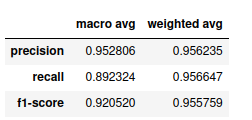
\includegraphics[scale = 0.75]{met_m1.png}
\caption{Metrics for model 1 }
\label{met_m1}
\end{figure}



\subsection{Model 2}

In this model, we perform pruning by restricting the depth. We take the maximum allowed depth as a hyperparameter and perform a grid search on possible values. The evolution of weighted f1-score on \textbf{validation set} with tree depth is shown in Figure \ref{depth_f1}. The highest score is obtained for a \textbf{depth of 9.} The performance of the model with a depth of 9 on validation set is shown in Figure \ref{met_m2}. The weighted averaged f1-score is \textbf{0.968. Clearly the model outperforms Model 1.}

\begin{figure}[tbh]
\centering
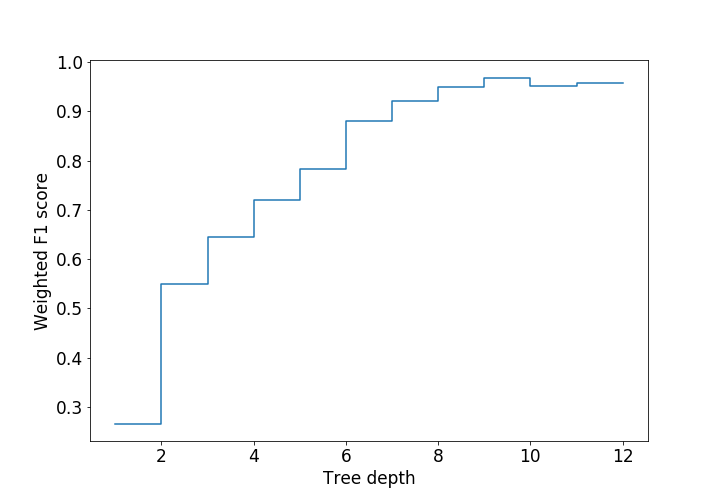
\includegraphics[scale = 0.34]{depth_f1.png}
\caption{Evolution of f1-score with tree depth}
\label{depth_f1}
\end{figure}

\begin{figure}[tbh]
\centering
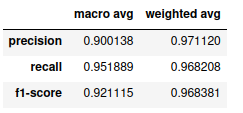
\includegraphics[scale = 0.75]{met_m2.png}
\caption{Metrics for model 2 }
\label{met_m2}
\end{figure}

\subsection{Model 3}

In this model, we perform bagging of decision trees. Since we are taking an ensemble, we can allow each tree to grow in an unrestricted fashion. We train each tree on a random subset of the training data, with the subset size being half of the total dataset size. We take the number of trees as a hyperparameter and perform a grid search on possible values. The evolution of weighted f1-score on \textbf{validation set} with number of trees is shown in Figure \ref{B_f1}. The highest score is obtained for a \textbf{tree count of 50.} The performance of the model with number of trees set to 50 on validation set is shown in Figure \ref{met_m3}. The weighted averaged f1-score is \textbf{0.962. Clearly the model outperforms Model 1, but is not as good as Model 2.}

\begin{figure}[tbh]
\centering
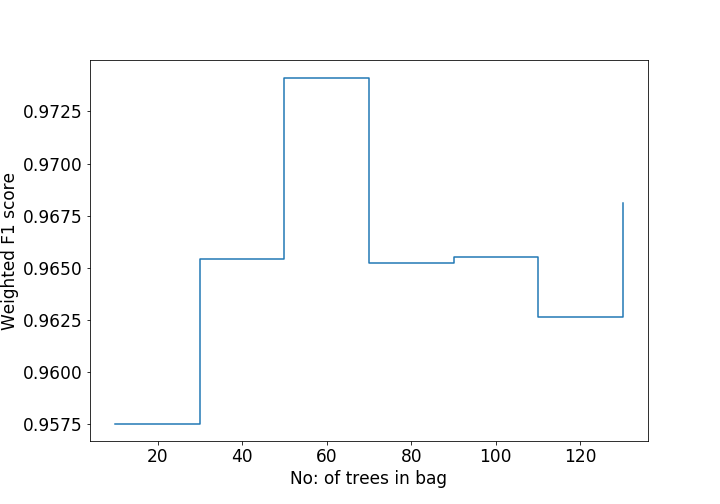
\includegraphics[scale = 0.34]{b_f1.png}
\caption{Evolution of f1-score with number of trees}
\label{B_f1}
\end{figure}

\begin{figure}[tbh]
\centering
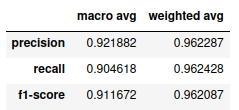
\includegraphics[scale = 0.75]{met_m3.png}
\caption{Metrics for model 3 }
\label{met_m3}
\end{figure}

\subsection{Best Model}

From the above analysis, we conclude that Model 2 performs the best. Hence, we train a decision tree of depth 9 on the whole dataset consisting of training set and the validation set. We then evaluate this on the test set. The metrics for this final model is given in Figure \ref{met_best} and the confusion matrix is given in Figure \ref{cf_matrix}. 

To get a sense of the importance of features, we also calculate the feature importance scores of each feature using an in-built method provided by scikit-learn. Essentially, the importance of a feature is computed as the (normalized) total reduction of the criterion brought by that feature. It is also known as the Gini importance. A plot showing the feature importance scores is given in Figure \ref{feature_imp}. \textbf{It can be seen that safety rating is the most important feature, whereas number of doors is the least important feature.} It is noteworthy that this agrees with our analysis during the exploratory phase.

\begin{figure}[tbh]
\centering
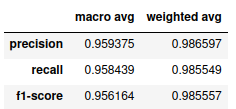
\includegraphics[scale = 0.75]{met_best.png}
\caption{Metrics for the best model }
\label{met_best}
\end{figure}

\begin{figure}[tbh]
\centering
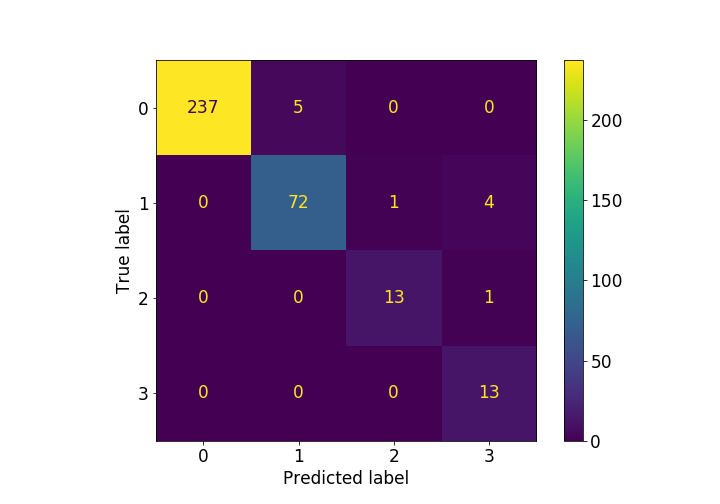
\includegraphics[scale = 0.34]{cfmatrix.png}
\caption{Confusion matrix for the best model}
\label{cf_matrix}
\end{figure}

\begin{figure}[tbh]
\centering
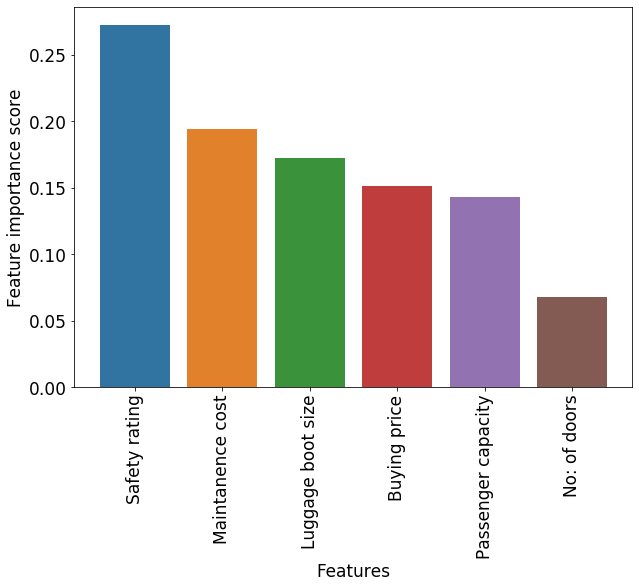
\includegraphics[scale = 0.34]{feature_imp.png}
\caption{Feature importance scores}
\label{feature_imp}
\end{figure}


\section{Conclusions}

From our extensive analysis of the given dataset using decision tree classifier, we arrive at the following conclusions:

\begin{itemize}
    \item Decision tree classifier, despite having a very simple structure, performs reasonably well in the classification task and mimics human decision making process. 
    \item Decision trees are prone to overfitting. Hence, it is necessary to take remedial measures like pruning and bagging to overcome this issue.
    \item Accuracy may not be a good measure of performance for imbalanced classification tasks. It is necessary to use metrics like weighted f1-score for such cases.
    \item Best performance is obtained after using pruning and setting the maximum depth to 9.
    \item Safety rating is found to be the most important feature whereas number of doors is found to be the least important feature, as was also observed during the initial qualitative analysis.
\end{itemize}



\section{Avenues for further research}

Decision classifier, despite working reasonably well, has a very simple structure which might not be sufficient in many cases. Using more sophisticated tree-based models like Random Forests might produce better results, though at the expense of interpretability. Doing some kind of feature preprocessing like PCA, to extract important features might also help. 



\nocite{*} % Print all references regardless of whether they were cited in the poster or not
\bibliographystyle{ieeetr}
\bibliography{sample} % Use the example bibliography file sample.bib


\end{document}

